\section{Kinematics}\label{sec:kinematics}
The two channels proposed to be studied are 
\begin{align}
ep\to e'p' \etaP  \label{eq:etaP} \\
ep\to e'p' \phi   \label{eq:phiP} \ ,
\end{align}
where $e$, $p$, $e'$, $p'$ are the incoming electron beam, target proton, scattered electron off of the beam and scattered proton, respectively. The quantities $\etaP$ and $\phi$ are the electro-produced mesons. The production mechanisms of such mesons have been already proposed in previous proposals~\cite{clas.proposal.eta,clas.proposal.phi} and are scheduled to run in conjunction with RunGroupA, the same run group requested for in this proposal.
The main decays studied for this proposal are:
\begin{align}
\etaP \rightarrow \gamma \gamma \to e^+e^- \gamma \label{eq:etaPconv} \\
\etaP \rightarrow \gamma \gamma^\star \to \gamma e^+e^- \label{eq:etaPDal} 
\end{align}
i.e. when a pseudoscalar meson, $P_p$($\eta'$), decays via two photons (Eq.~\ref{eq:etaPconv}) and one photon converts into an \epemT \ pair due to E.M. processes through matter, this is conventionally known as external conversions. This decay channel will he the main background contribution and in further discussed in SecXXX. The Dalitz decay, or internal conversion, is when the $P_p$($\eta'$) decays via a real photon and a virtual photon (Eq.~\ref{eq:etaPDal}), which decays into an \epemT \ pair.
\begin{align}
\phi \rightarrow  \eta \gamma \to \eta e^+e^- \label{eq:phiPconv} \\
\phi \rightarrow \eta  \gamma^\star \to \eta  e^+e^-\label{eq:phiPDal} \ ,
\end{align}
i.e. when a vector meson $V_p$($\phi$), decays via an \etaT \ and a photon(Eq.~\ref{eq:phiPconv}) and one photon converts into an \epemT \ pair. The Dalitz decay for the $\phi$ is when $V_p$($\phi$) decays via an $\eta$ and a virtual photon (Eq.~\ref{eq:phiPDal}), which decays into an \epemT \ pair.
Figure~\ref{fig:piz.alldecay} illustrates the Feynman diagrams for the pseudoscalar ``two photon decay'' and  ``Dalitz decay'', while Fig.~\ref{fig:phi.alldecay} illustrates the Feynman diagrams for the vector ``pseudoscalar photon decay'' and  ``Dalitz decay''.
 %Table~\ref{tab:pi0}. Figure~\ref{fig:piz.alldecay} illustrates the Feynman diagrams for the ``Two photon decay'' and the ``Dalitz decay''.
 \begin{figure}[h!]\begin{center}
 		\subfloat[Feynman Diagram of $\etaP$ Two Photon Decay][]{ %Feynman diagram of $\etaP$ two photon decay
 			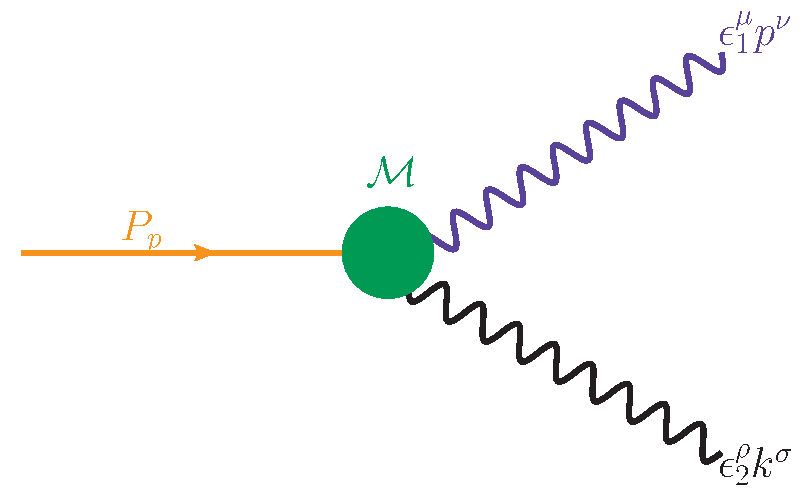
\includegraphics[width=0.4\columnwidth,height=0.75\qfigheight]{\grpath/decays/psudoscalar_gammagamma.pdf}\label{fig:piz.gamgam}
 		}
 		\quad
 		\subfloat[Feynman Diagram of $\etaP$ Dalitz Decay][]{ %Feynman diagram of $\etaP$ Dalitz decay
 			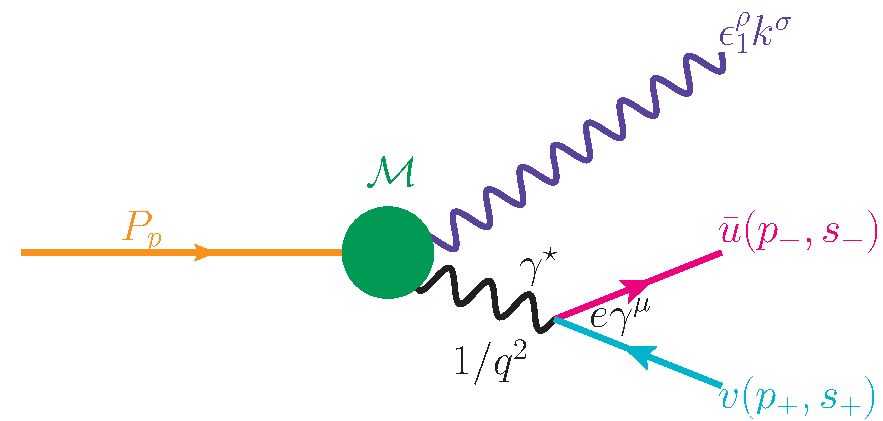
\includegraphics[width=0.45\columnwidth,height=0.75\qfigheight]{\grpath/decays/psudoscalar_dalitz.pdf}\label{fig:piz.dalitz}
 		}
 		\caption[Feynman diagram of $P_p$($\etaP$) two photon decay and Dalitz decay]{\label{fig:piz.alldecay}Feynman diagram of $P_p$($\etaP$) two photon decay~\subref{fig:piz.gamgam}, $\epsilon_1$ and $\epsilon_2$ are the polarizations, $p$ and $k$ are 4-momenta of the photons.  Feynman diagram of $P_p$($\etaP$) Dalitz decay~\subref{fig:piz.dalitz}, the variable $s_\pm$ are the spin helicities of the outgoing leptons $l^\pm$ with 4-momenta $p_{\pm}$ and $\epsilon$ is the polarization of the outgoing photon with 4-momenta $k$. In both diagrams $\mathcal{M}$ is the form factor.}
\end{center}\end{figure}
\begin{figure}[h!]\begin{center}
 	 		\subfloat[Feynman Diagram of $\phi \to \eta \gamma$ Decay][]{ %Feynman diagram of $\etaP$ two photon decay
 	 			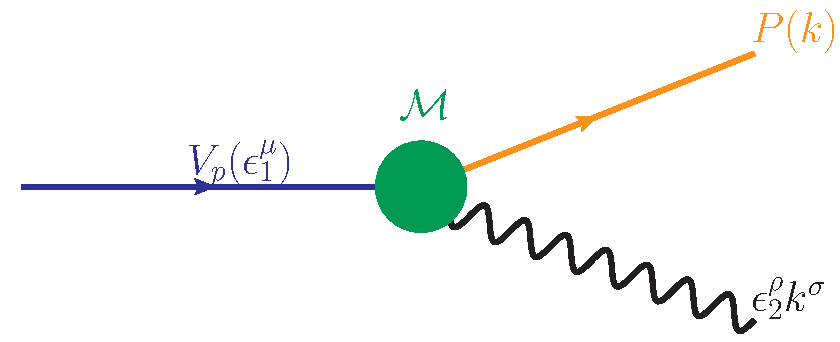
\includegraphics[width=0.4\columnwidth,height=0.75\qfigheight]{\grpath/decays/vector_gammapseudo.pdf}\label{fig:phi.etagam}
 	 		}
 	 		\quad
 	 		\subfloat[Feynman Diagram of $\phi$ Dalitz Decay][]{ %Feynman diagram of $\etaP$ Dalitz decay
 	 			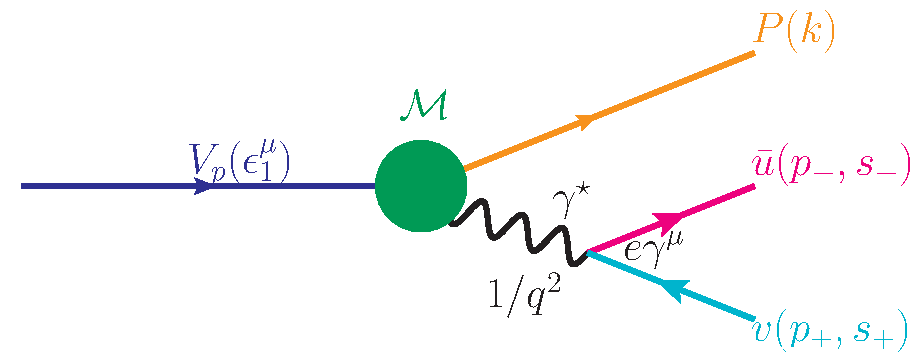
\includegraphics[width=0.45\columnwidth,height=0.75\qfigheight]{\grpath/decays/vector_dalitz.pdf}\label{fig:phi.dalitz}
 	 		}
 	 		\caption[Feynman diagram of $V_p$($\phi$) decays]{\label{fig:phi.alldecay}Feynman diagram of $V_p$($\phi$) deacys. Notation same as in Fig.~\ref{fig:piz.alldecay}.}
\end{center}\end{figure}
 A full derivation of the external conversion and Dalitz decay are given in the Appendix~\ref{sec:app}.
  \subsection{The Dalitz Decay}
  The Dalitz decay of mesons is dependent on the spin of the meson. For pseudoscalar meson the decay rate is derived in~\ref{sec:dalitzdecay} and is expressed as:
  \begin{align}\label{eq:eegff.finalkroll_II}
  \frac{d\Gamma_{\epem \gamma}}{\Gamma_{\gamma\gamma} dq^2} = \frac{2 \alpha}{3 \pi} \frac{1}{q^2} \left( 1- \frac{q^2}{m_p^2}\right)^3 \left( 1+ \frac{2m_l^2}{q^2}\right) \left( 1- \frac{4m_l^2}{q^2}\right)^{\frac{1}{2}} 
  \end{align}
  which is the Kroll-Wada equation founded in~\cite{KrollWada,landsberg}. For vector mesons, the decay rate can be expressed as:
  \begin{align}
  \frac{d\Gamma}{\Gamma_{\eta\gamma} dq^2} = \frac{\alpha}{3 \pi} \frac{1}{q^2} \left( \left(1+ \frac{q^2}{m_{\phi}^2 - m_{\eta}^2} \right)^2 - \frac{4 m_{\phi}^2 q^2}{m_{\phi}^2 - m_{\eta}^2}\right)^\frac{3}{2} \left( 1+ \frac{2m_l^2}{q^2}\right) \left( 1- \frac{4m_l^2}{q^2}\right)^{\frac{1}{2}} \ ,
  \end{align}
  as derived as~\cite{landsberg}:
   An example of QED expectation for \etaTP  \ and $phi$ is shown in Fig.~\ref{fig:dalitz_compare}.
  \subsection{Form Factor}
  The form factor ${M}_P(p^2,k^2=0)$ or ${M}_P(p_{1}^2,p_{2}^2)$  can be written as follows:
  \begin{align}
  {M}_P \to {M}_P \times \left|F(q^2)\right| \ ,
  \end{align}
  where $M_p$ is the decay constant of two photons or $\eta$ photon (as mentioned in Sec.~\ref{sec:piz.gg}), while $\left|F(q^2)\right|$ is called the transition form factor, which defines the electromagnetic space structure of the meson, therefore for the $\etaP \to e^+e^- \gamma$ the decay rate modifies as;
  \begin{align}\label{eq:eegff.final}
  \frac{d\Gamma_{\epem \gamma}}{\Gamma_{\gamma\gamma} dq^2} = \frac{2 \alpha}{3 \pi} \frac{1}{q^2} \left( 1- \frac{q^2}{m_p^2}\right)^3 \left( 1+ \frac{2m_l^2}{q^2}\right) \left( 1- \frac{4m_l^2}{q^2}\right)^{\frac{1}{2}} \left|F(q^2)\right|^2 \ ,
  \end{align}
  ,which is the Kroll-Wada equation founded in~\cite{KrollWada}, while the $\phi \to \eta e^+e^-$ decay rate modifies as;
  \begin{align}
  \frac{d\Gamma_{\eta \epem}}{\Gamma_{\eta\gamma} dq^2} = \frac{\alpha}{3 \pi} \frac{1}{q^2} \left( \left(1+ \frac{q^2}{m_{\phi}^2 - m_{\eta}^2} \right)^2 - \frac{4 m_{\phi}^2 q^2}{m_{\phi}^2 - m_{\eta}^2}\right)^\frac{3}{2} \left( 1+ \frac{2m_l^2}{q^2}\right) \left( 1- \frac{4m_l^2}{q^2}\right)^{\frac{1}{2}} \left|F(q^2)\right|^2 \ ,
  \end{align}
  
  The value of $\left|F(q^2)\right|$ can be directly measured by comparison of the differential cross section with that of Q.E.D. pointlike differential cross section i.e.
  \begin{align}
  \frac{d\sigma}{dq^{2}} = \left[\frac{d\sigma}{dq^{2}}\right]_{\text{pointlike}}\left| F(q^{2})\right| ^{2}\nonumber \ ,
  \end{align}
  or by performing a line shape analysis on the $l^{+}l^{-}$ invariant system using assumptions on the structure of $\left|F(q^2)\right|$. One such assumption for $\left|F(q^2)\right|$ is the dipole approximation, from the Vector Dominance Model (VMD), in which 
  \begin{align}
  F(q^{2}) = \frac{\Lambda^2(\Lambda^2 + \gamma^2)}{(\Lambda^{2} - q^2) + \Lambda^2\gamma^2 } \nonumber
  \end{align}
  where the parameters $\Lambda$ and $\gamma$ correspond to the mass and width of the Breit-Wigner shape for the effective contributing vector meson. A first approximation is that $\Lambda \approx M_{\rho} \approx 0.7$~GeV and $\gamma \approx \Gamma_{\rho}  \approx 0.12$~GeV. A comparison showing the QED spectra and the deviation from QED using the VMD parameterization is shown in Fig.~\ref{fig:dalitz_compare} for \etaTP  \ and $\phi$.
 \begin{figure}[h!]\begin{center}
 		\subfloat[$\etaP$ Dalitz spectra][]{ %Feynman diagram of $\etaP$ two photon decay
 			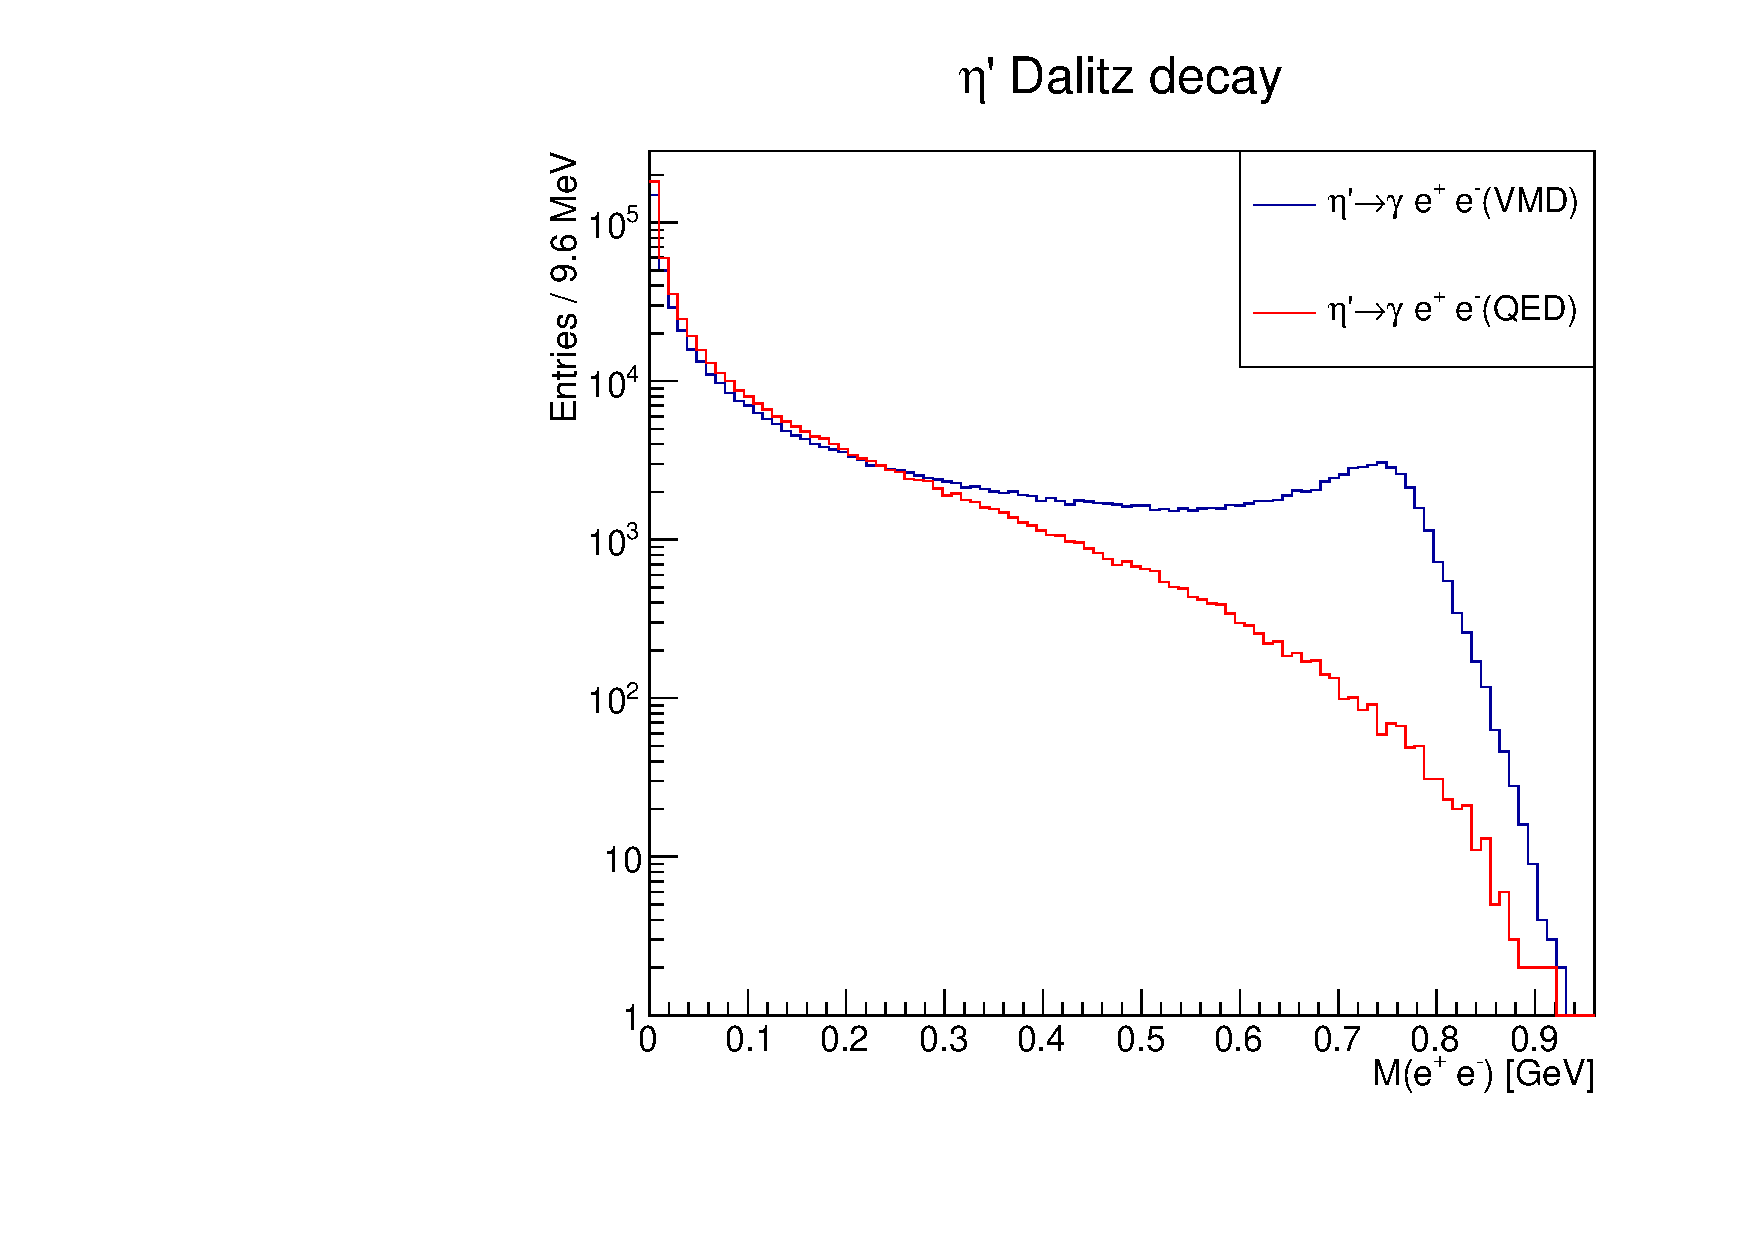
\includegraphics[width=0.8\columnwidth,height=1.0\qfigheight]{\grpath/decays/etaP_Dalitz_QED_FF_comparePlot.pdf}\label{fig:etap_dalitz_conpare}
 		}
 		%\quad 
 		\\
 		\subfloat[$\phi$ Dalitz  spectra][]{ %Feynman diagram of $\etaP$ Dalitz decay
 			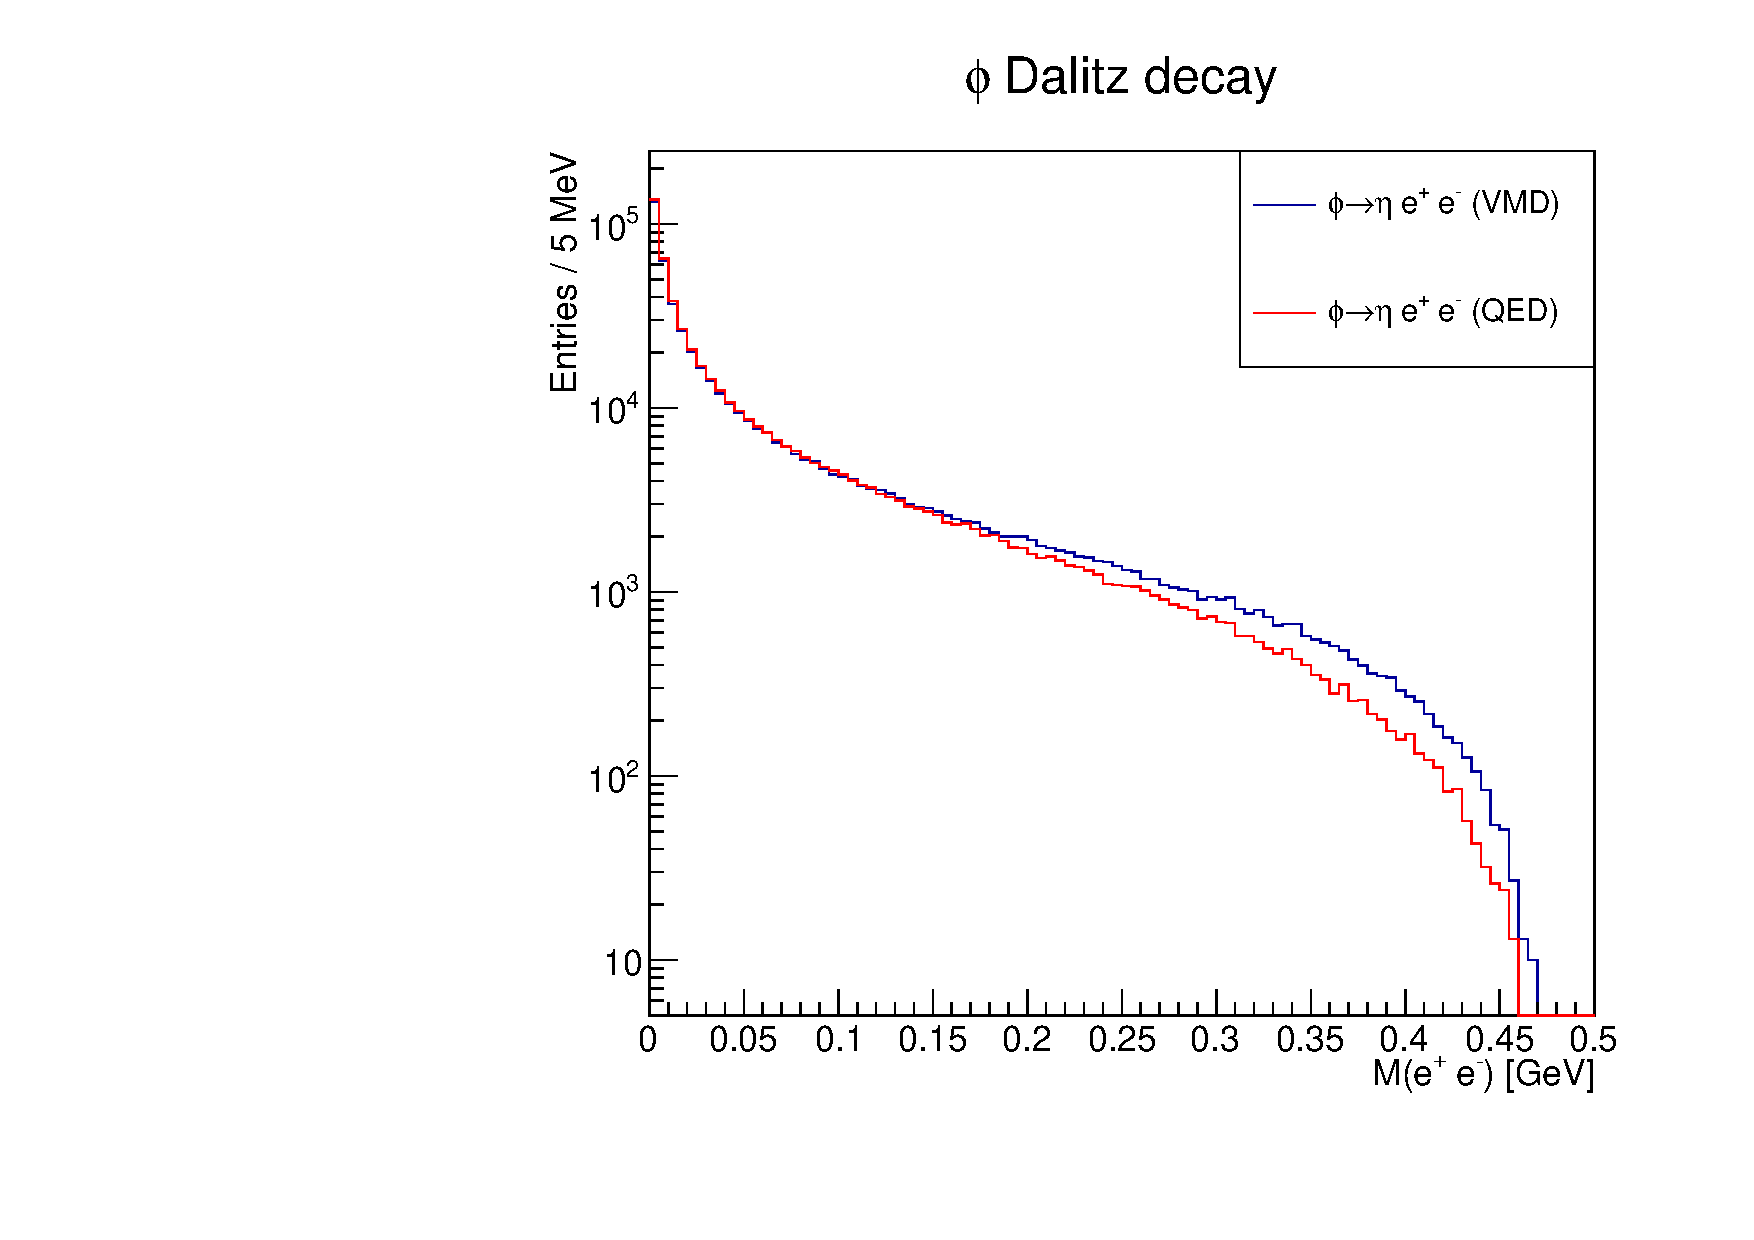
\includegraphics[width=0.8\columnwidth,height=1.0\qfigheight]{\grpath/decays/phi_Dalitz_QED_FF_comparePlot.pdf}\label{fig:phi_dalitz_compare}
 		}
 		\caption[Dalitz  for \etaTP \ and $\phi$]{\label{fig:dalitz_compare}Example of Dalitz spectra for \etaTP \ using only QED(red) and the deviation from QED using the VMD parameterization(blue) with 500K Dalitz events generated~\subref{fig:etap_dalitz_w_conversion}.  Example of Dalitz  spectra for $\phi$ using only QED(red) and the deviation from QED using the VMD parameterization(blue)  with 500K Dalitz events generated~\subref{fig:phi_dalitz_w_conversion}. }
 	\end{center}\end{figure}
 	 
\subsection{Photon Conversion to \epemT Pairs}\label{sec:intro.conversion}
When a photon travels through matter at energies greater than 100~MeV, it can convert into an electron-positron pair. The process of pair production, $\gamma Z \rightarrow Ze^{+}e^{-}$, occurs when a photon with $E_0 > 2 m_e c^2$ converts into an electron and a positron. The cross section for this process can be written as;
\begin{equation}\label{pair_crosssection}
\sigma_{\gamma\rightarrow e^+e^-} =  \frac{A}{N_{A} \rho \lambda_\gamma}  \ ,\ \lambda_\gamma = \frac{9}{7}X_0
\end{equation}
where $\lambda$ is the interaction length, or mean free path, $\rho$ is the density of the material, $N_A$ is Avogadro's number and $A$ is the atomic mass of the material. The probability of pair production to occur is solely based on $X_{0}$, the radiation length of the medium and this probability can be expressed as;
\begin{equation}
\frac{dP}{dx} = \frac{1}{\lambda_\gamma}\exp(\frac{-x}{\lambda_\gamma}) \ .
\end{equation}
%
%
Using the ratio, $\frac{\Gamma_{\etaP \to e^+e^- \gamma}}{\Gamma_{\etaP \to \gamma \gamma}} = 2.13\cdot 10^{-2}$, that has been preliminary measured by CLAS, which is consistent with~\cite{BESIII}, the probability of pair production when a photon, from the $\etaP \to \gamma \gamma$ decay, traveling though 5~cm of liquid hydrogen, $\ell$H$_2$, is shown in Fig.~\ref{fig:conversion} as well as the number of $\etaP \to \gamma \gamma \rightarrow e^+e^- \gamma$ / $100 \etaP \rightarrow e^+e^- \gamma$. 
\begin{figure}[h!]\begin{center}
	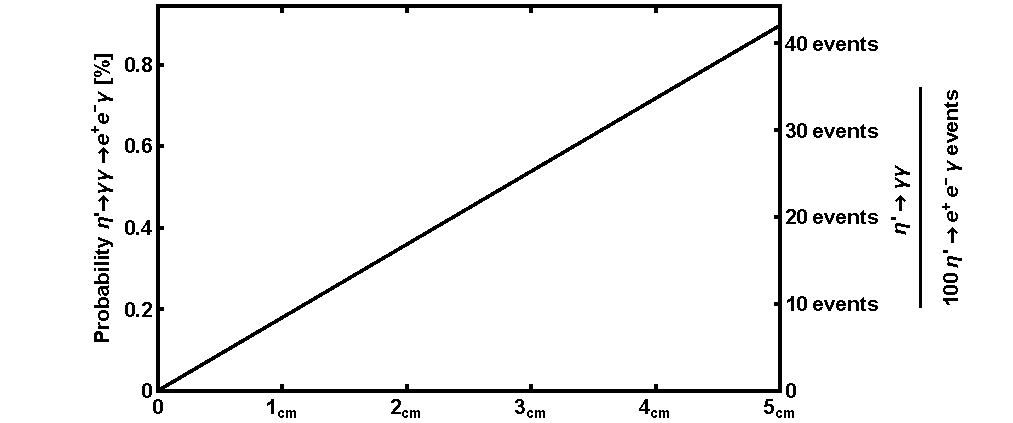
\includegraphics[width=\figwidth,height=\qfigheight]{\grpath/decays/cmplot.pdf}
	\caption[Probability of pair production, $\gamma \to$\epemT, as a function of distance in liquid hydrogen]{\label{fig:conversion}{(Left axis)Probability of pair production, $\gamma \to$\epemT; (Right axis) number of $\etaP \to \gamma \gamma \rightarrow e^+e^- \gamma$ / $100 \etaP \rightarrow e^+e^- \gamma$ as a function of distance in liquid hydrogen.}}
\end{center}\end{figure}
	Since CLAS12 has a vertex resolution of $\approx$1~mm the probability of pair production traveling through 10~mm is shown in Fig.~\ref{fig:conversionmm}. Therefore, a 1~mm cut on the primary vertex will yield a contamination of $\approx$ one externally converted \epemT from $\etaP \to \gamma \gamma \rightarrow e^+e^- \gamma$ per Dalitz decays $100 \etaP \rightarrow e^+e^- \gamma$
\begin{figure}[h!]\begin{center}
	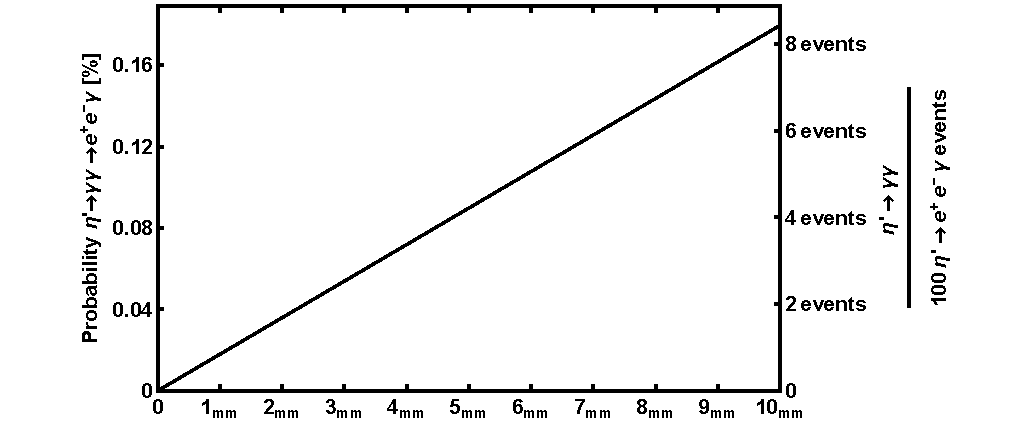
\includegraphics[width=\figwidth,height=\qfigheight]{\grpath/decays/mmplot.pdf}
	\caption[Probability of pair production, $\gamma \to$\epemT, as a function of distance in liquid hydrogen]{\label{fig:conversionmm}{(Left axis)Probability of pair production, $\gamma \to$\epemT; (Right axis) number of $\etaP \to \gamma \gamma \rightarrow e^+e^- \gamma$ / $100 \etaP \rightarrow e^+e^- \gamma$ as a function of distance in liquid hydrogen.}}
\end{center}\end{figure}
These type of subprocess mimics the Dalitz decay  $\etaP \to e^+e^- \gamma$, described in Sec.~\ref{sec:dalitzdecay}. Since there are two photons with equal probability of conversion for $\etaP \to \gamma \gamma$, the total probabilities shown is for when either photon externally converts.
Using the ratio, $\frac{\Gamma_{\phi \to e^+e^- \eta}}{\Gamma_{\phi \to \gamma \eta}} = 9.58\cdot 10^{-2}$~\cite{pdg2014}, the probability of pair production when a photon, from the $\phi \to \gamma \eta$ decay, traveling though 5~cm of liquid hydrogen, $\ell$H$_2$, is shown in Fig.~\ref{fig:conversionphi} as well as the number of $\phi \to \gamma \eta \rightarrow e^+e^- \eta$ / $100 \phi \rightarrow e^+e^- \eta$. 
\begin{figure}[h!]\begin{center}
	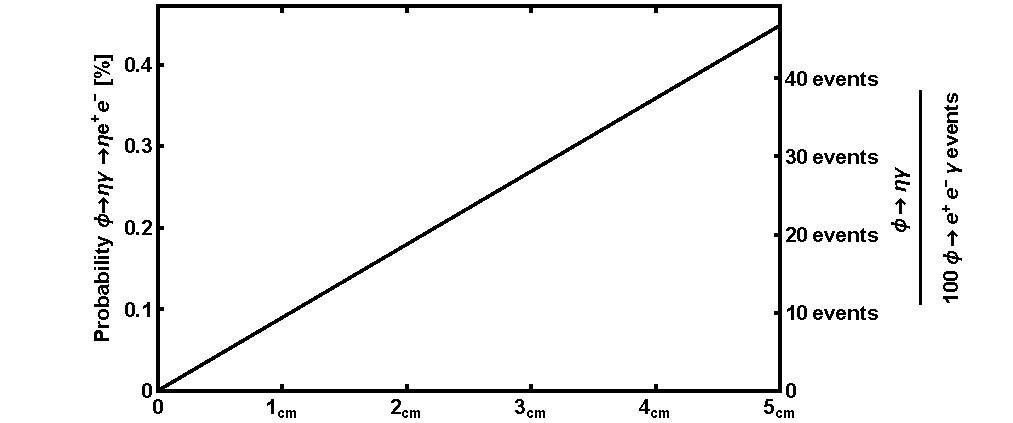
\includegraphics[width=\figwidth,height=\qfigheight]{\grpath/decays/phicmplot.pdf}
	\caption[Probability of pair production, $\gamma \to$\epemT, as a function of distance in liquid hydrogen]{\label{fig:conversionphi}{(Left axis)Probability of pair production, $\gamma \to$\epemT; (Right axis) number of $\phi \to \gamma \eta \rightarrow e^+e^- \eta$ / $100 \phi \rightarrow e^+e^- \eta$ as a function of distance in liquid hydrogen.}}
\end{center}\end{figure}
			Since CLAS12 has a vertex resolution of $\approx$1~mm the probability of pair production traveling through 10~mm is shown in Fig.~\ref{fig:conversionmm}. Therefore, a 1~mm cut on the primary vertex will yield a contamination of $\approx$ one externally converted \epemT from $\phi \to \gamma \eta \rightarrow e^+e^- \eta$ per Dalitz decays $100 \phi \rightarrow e^+e^- \eta$
\begin{figure}[h!]\begin{center}
	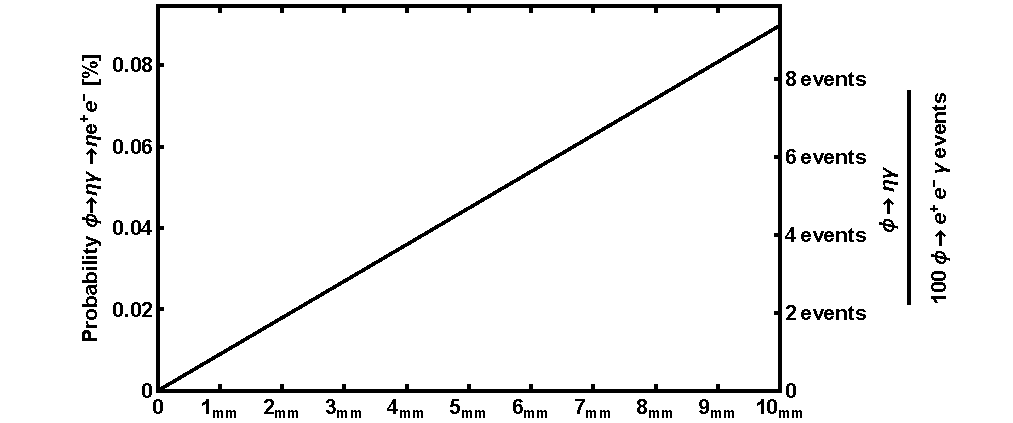
\includegraphics[width=\figwidth,height=\qfigheight]{\grpath/decays/phimmplot.pdf}
	\caption[Probability of pair production, $\gamma \to$\epemT, as a function of distance in liquid hydrogen]{\label{fig:conversionphimm}{(Left axis)Probability of pair production, $\gamma \to$\epemT; (Right axis) number of $\phi \to \gamma \eta \rightarrow e^+e^- \eta$ / $100 \phi \rightarrow e^+e^- \eta$ as a function of distance in liquid hydrogen.}}
\end{center}\end{figure}
From multiple scattering effects the \epemT \ from a converted photon will obtain a mass distribution. Simulations of photons from \etaTP \ and $\phi$ radiative decays traversing through 1~mm of $\ell H_2$  show that the \epemT can obtain a maximum mass of $\sim 0.14$~GeV.		
\begin{figure}[h!]\begin{center}
		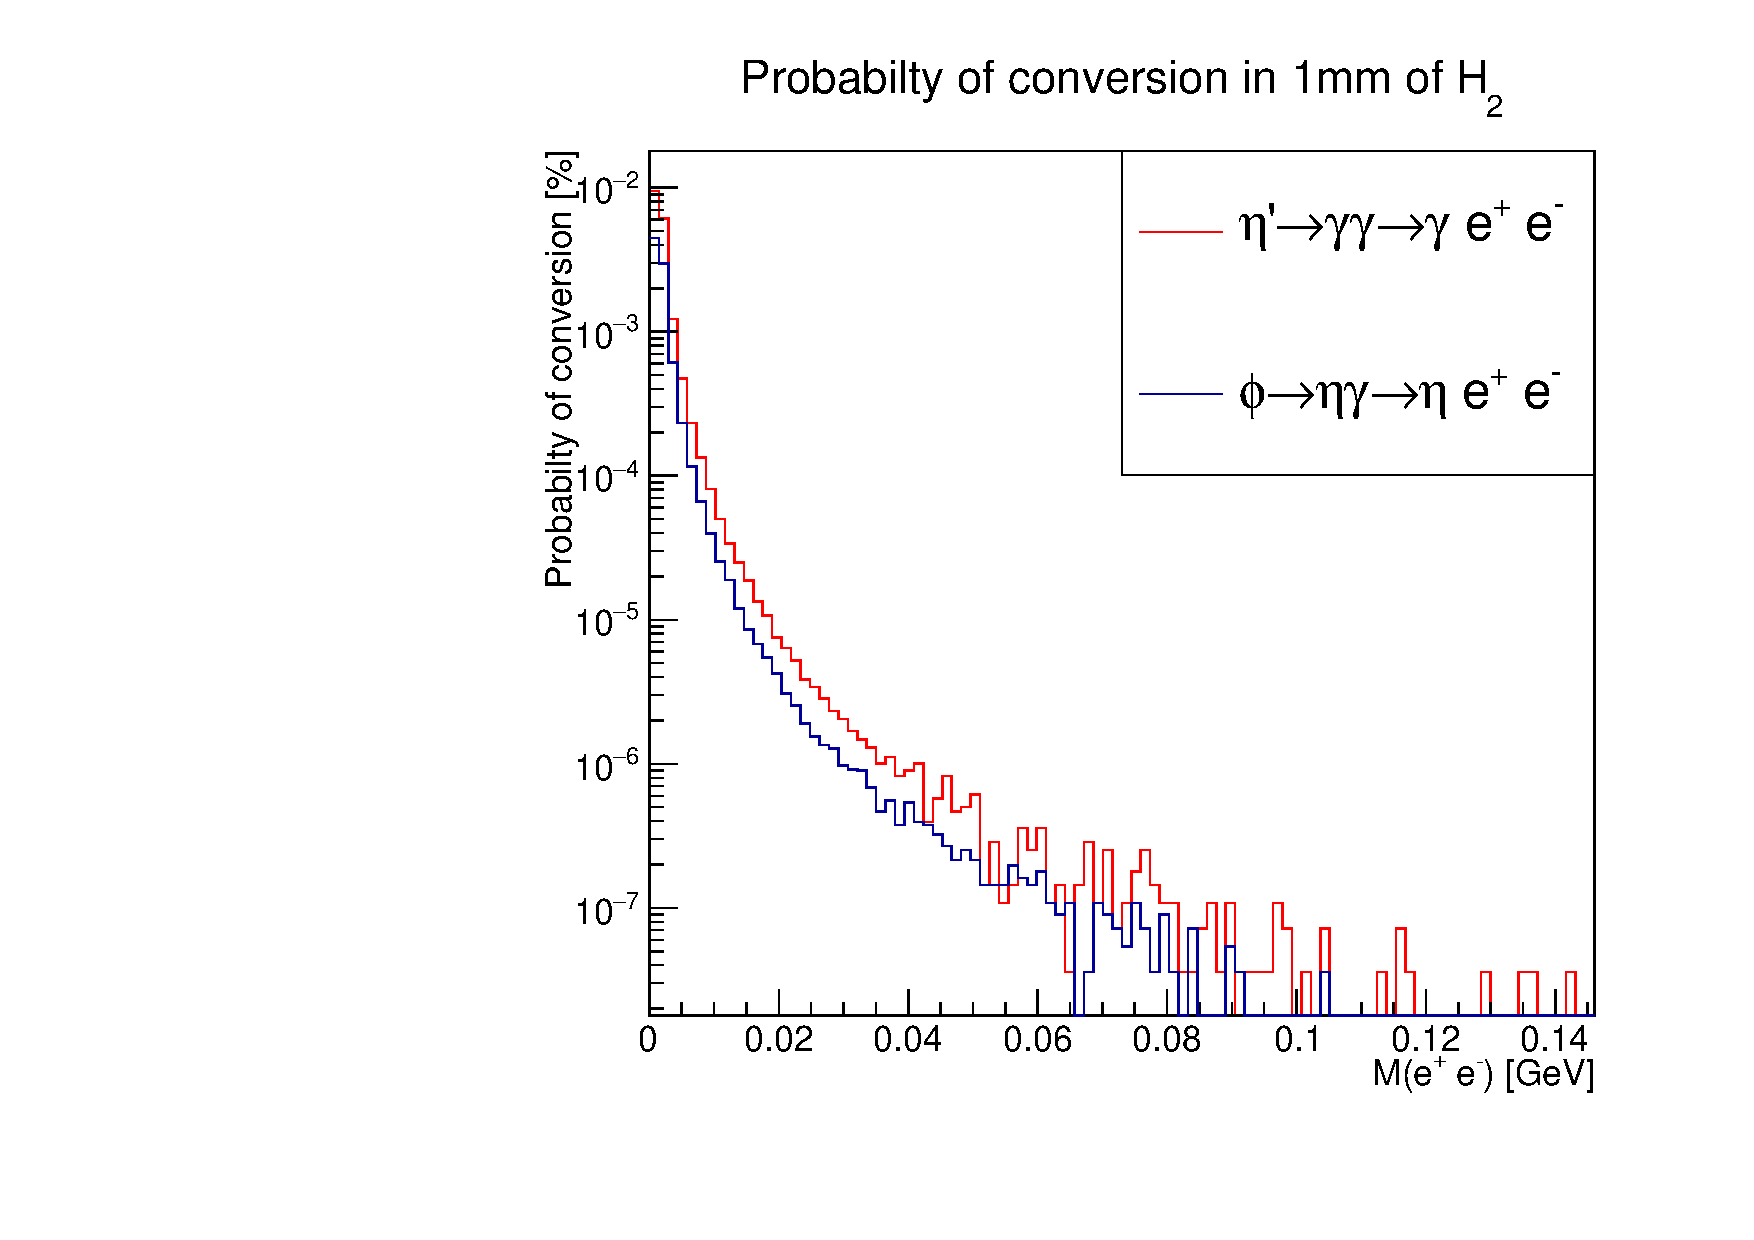
\includegraphics[width=\figwidth,height=1.2\qfigheight]{\grpath/decays/etaP_phi_conversionPlot.pdf}
		\caption[Probability of pair production, $\gamma \to$\epemT, as a function of $M(\epem)$]{\label{fig:conversion_inM}{Probability of pair production in 1~mm of  $\ell H_2$ for $\etaP \to \gamma \gamma $ and $\phi \to \gamma \eta$  vs. $M(\epem)$}}
\end{center}\end{figure}
 \subsection{Summary}
 The $\gamma \gamma$ decay and the $\gamma^\star \gamma$ decay have different branching ratios as do the decays $\gamma \eta$ decay and the $\gamma^\star \eta$. This difference is attributed to the factor of $\alpha$ along with a $q^2$ dependence calculated in the Dalitz decay. However, due to the probability of a photon converting into an electron-positron pair in $\ell$H$_2$, the total amount of \epemT pairs produced via photon conversion can contaminate the measurement of the form factor. The CLAS detector will have vertex resolution of $\sim$1~mm, therefore the amount of contamination of externally converted pairs will be minimized by the vertex position of the \epemT pair. An example of the total contamination, in the Dalitz spectrum, from external conversion within 1~mm of the primary vertex can be seen in Fig.~\ref{fig:dalitz_w_conversion}.
 \begin{figure}[h!]\begin{center}
 		\subfloat[$\etaP$ Dalitz and conversion spectra][]{ %Feynman diagram of $\etaP$ two photon decay
 			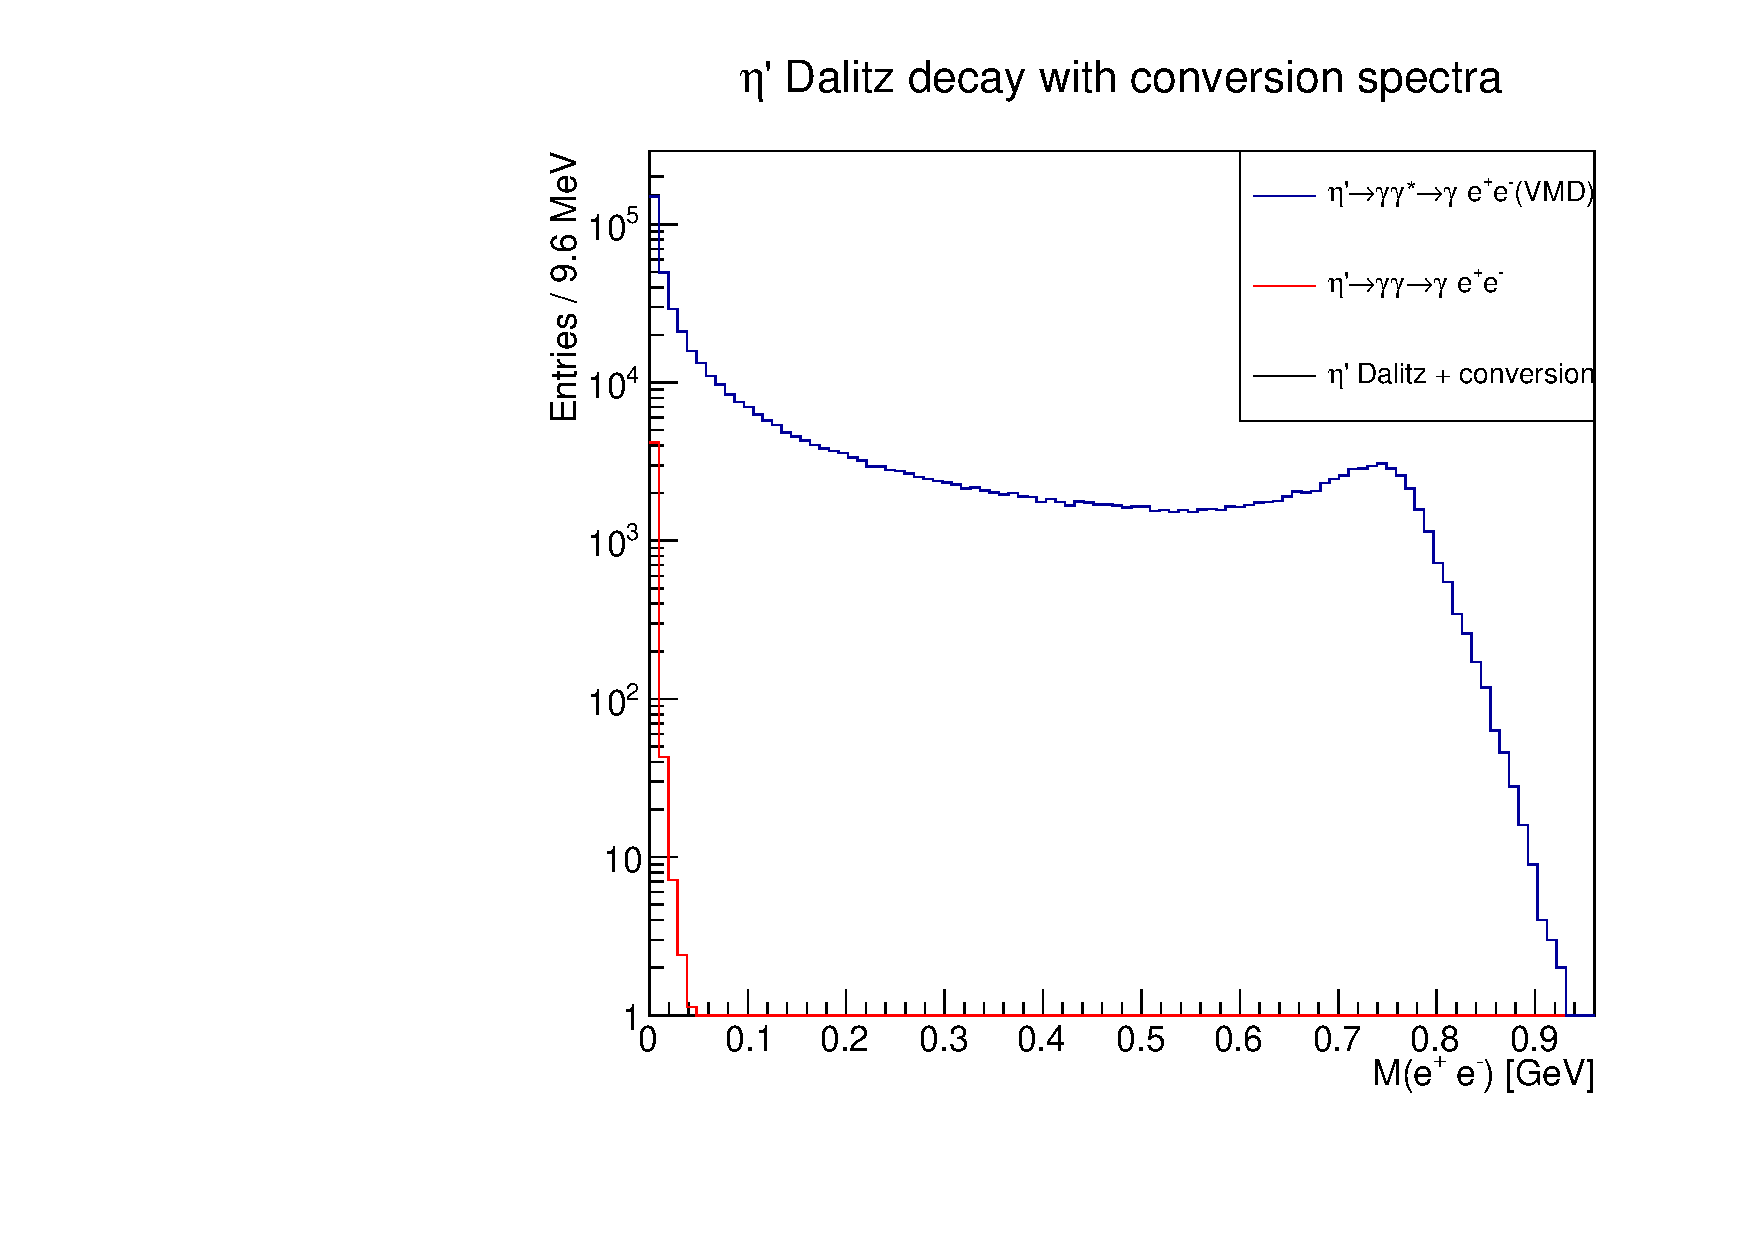
\includegraphics[width=0.8\columnwidth,height=1.0\qfigheight]{\grpath/decays/etaP_Dalitz_decay_with_conversion_spectra.pdf}\label{fig:etap_dalitz_w_conversion}
 		}
 		%\quad 
 		\\
 		\subfloat[$\phi$ Dalitz and conversion spectra][]{ %Feynman diagram of $\etaP$ Dalitz decay
 			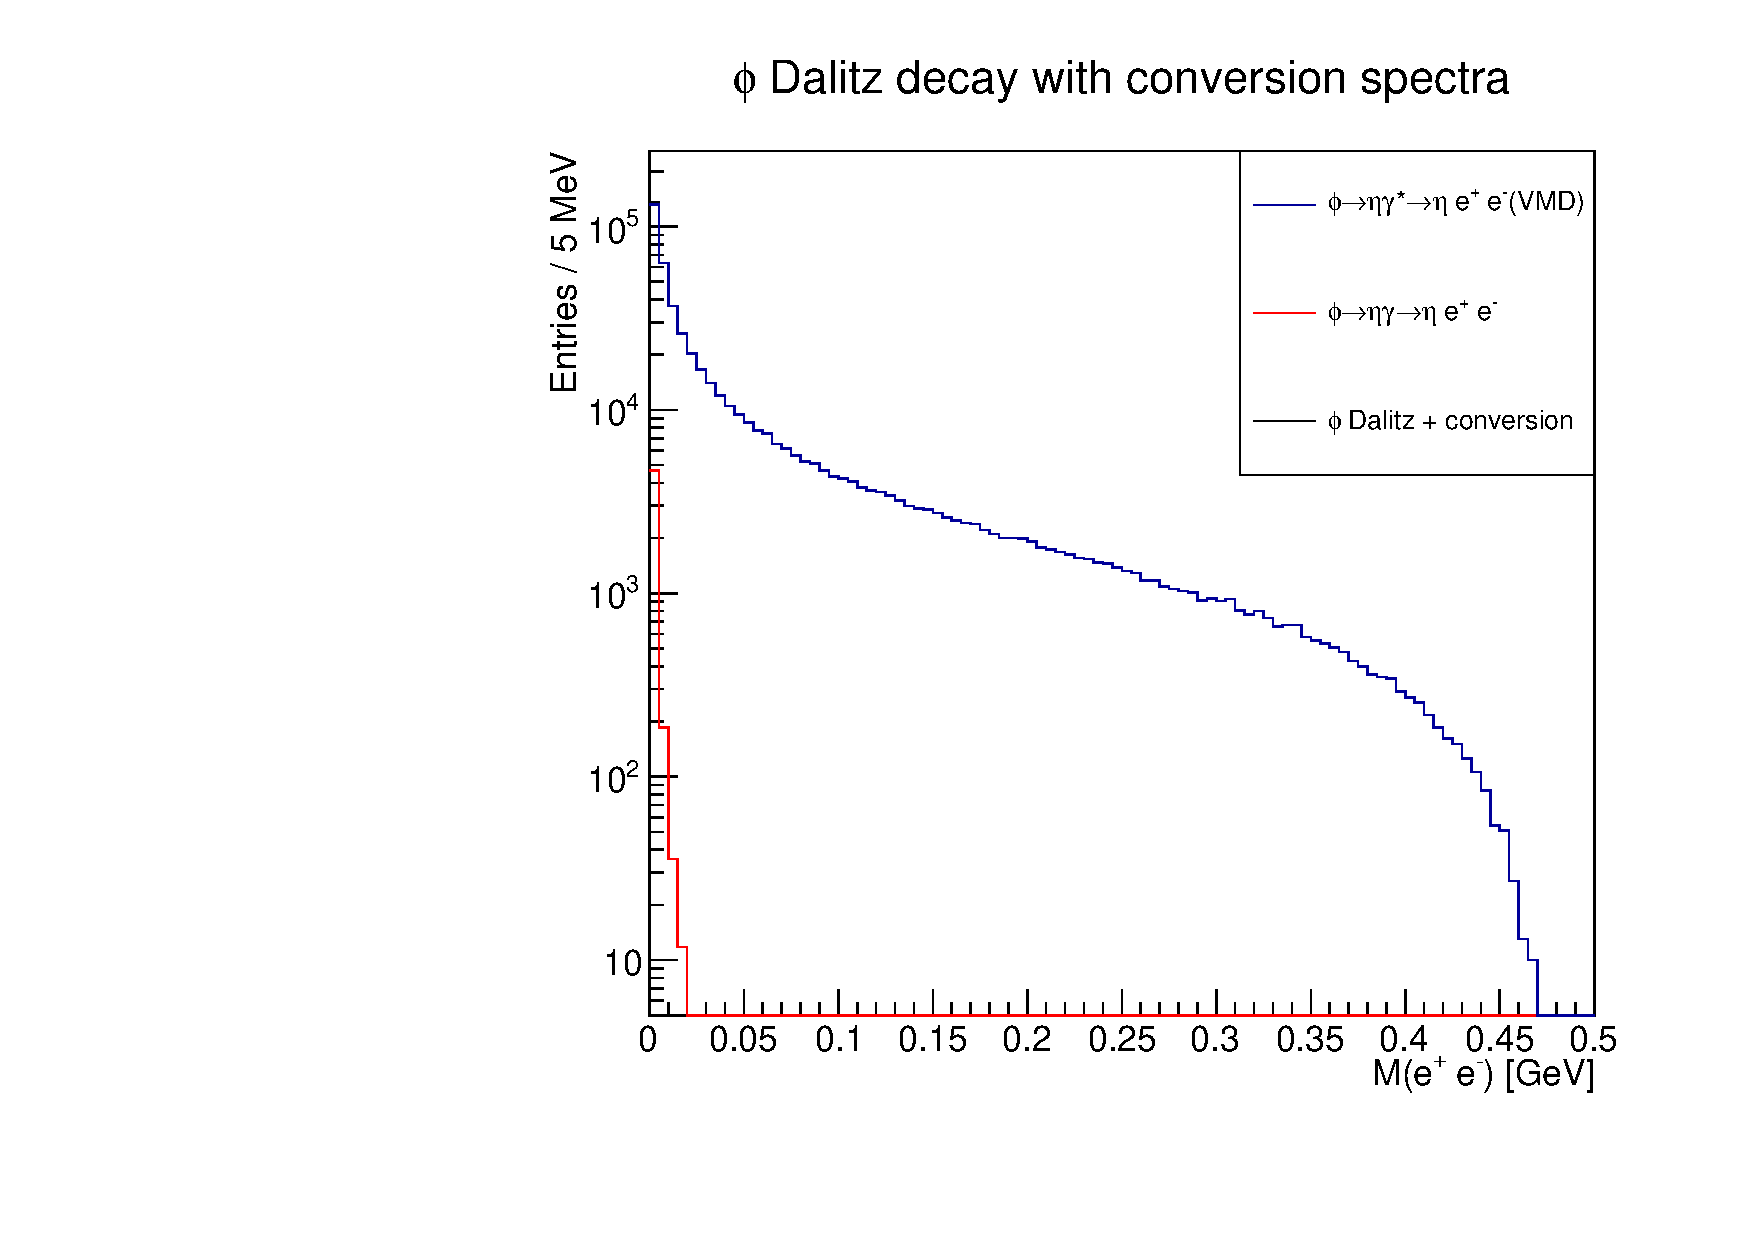
\includegraphics[width=0.8\columnwidth,height=1.0\qfigheight]{\grpath/decays/phi_Dalitz_decay_with_conversion_spectra.pdf}\label{fig:phi_dalitz_w_conversion}
 		}
 		\caption[Dalitz and conversion spectra for \etaTP \ and $\phi$]{\label{fig:dalitz_w_conversion}Example of Dalitz and conversion spectra for \etaTP \ with 500K Dalitz events generated and $\sim 2.35 \cdot 10^7$ $\etaP \to \gamma \gamma$ generated~\subref{fig:etap_dalitz_w_conversion}.  Example of Dalitz and conversion spectra for $\phi$  with 500K Dalitz events generated and $\sim 5.7 \cdot 10^7$ $\phi \to \eta \gamma$ generated ~\subref{fig:phi_dalitz_w_conversion}. }
\end{center}\end{figure}

  
  
  